\chapter{Appendix of Chapter~\ref{chap:mv-sto}}
\label{ap:mv-sto}

\minitoc

\begin{noaddcontents}
\section{About \Cref{chap:mv-sto:eq:lacasse}}
\label{ap:mv-sto:sec:algolacasse}

For the sake of completeness, we prove the bound $\Risk_{\Dp}(\MVQ) \le 2b_{\Dp}^{N}(\Q)$ in the following lemma.

\begin{lemma} For any distribution $\Dp$ on $\X\times\Y$, for any hypothesis set $\H$, for any distribution $\Q$ on $\H$, for any $N\in\Nbb_{*}$, we have
\begin{align*}
    \Risk_{\Dp}(\MVQ) &\le 2b_{\Dp}^{N}(\Q)\\
    &= 2\EE_{(\x,\y)\sim\Dp}\!\!\LB\sum_{j=\lceil\frac{N}{2}\rceil}^N\!\binom{N}{j}\! \LB\frac{1}{2}\LP1{-}\OmMaQ(\x,\y)\RP\RB^j\! \LB1{-}\frac{1}{2}\LP1{-}\OmMaQ(\x,\y)\RP\RB^{(N-j)}\RB.
\end{align*}
\label{ap:mv-sto:lemma:lacasse}
\end{lemma}
\begin{proof}
The proof is based on \citet{LacasseLavioletteMarchandTurgeonBoutin2010}.
Note that for a given example $(\x,\y)\sim\Dp$ \st $\OmMaQ(\x,\y)=0$, we have 
\begin{align*}
    \underbrace{\sum_{j=\lceil\frac{N}{2}\rceil}^N\binom{N}{j} \LB\frac{1}{2}\LP1-\OmMaQ(\x,\y)\RP\RB^j \LB1-\frac{1}{2}\LP1-\OmMaQ(\x,\y)\RP\RB^{(N-j)}}_{\defeq \heartsuit^{N}_{\Q}(\x,\y)} \ge \frac{1}{2}.
\end{align*}
Moreover, $\heartsuit^{N}_{\Q}(\x,\y)$ is monotonically decreasing in $\OmMaQ(\x,\y)$.
From these two properties, we have for a given example $(\x,\y)\sim\Dp$ \st $\OmMaQ(\x,\y)\le 0$
\begin{align*}
    \underbrace{\indic\LB \OmMaQ(\x,\y)\le 0 \RB}_{= 1} \le 2\heartsuit^{N}_{\Q}(\x,\y),
\end{align*}
and for a given example $(\x,\y)\sim\Dp$ \st $\OmMaQ(\x,\y)> 0$
\begin{align*}
    \underbrace{\indic\LB \OmMaQ(\x,\y)\le 0 \RB}_{= 0} \le 2\heartsuit^{N}_{\Q}(\x,\y).
\end{align*}
Hence, we can deduce that
\begin{align*}
    \Risk_{\Dp}(\MVQ) \le \EE_{(\x,\y)\sim\Dp}\indic\LB \OmMaQ(\x,\y)\le 0 \RB \le 2\EE_{(\x,\y)\sim\Dp}\heartsuit^{N}_{\Q}(\x,\y) = 2b_{\Dp}^{N}(\Q).
\end{align*}
\end{proof}

Based on \Cref{ap:mv-sto:lemma:lacasse}, we are now able to prove a PAC-Bayesian bound on the majority vote's true risk based on the surrogate $b_{\Dp}^{N}(\Q)$.
Note that \citet{LacasseLavioletteMarchandTurgeonBoutin2010} prove a \citeauthor{Catoni2007}-like bound while our work is based on a \citeauthor{Seeger2002}-like one.
Our bound avoids using a parameter $c\ge 0$ required in \citeauthor{Catoni2007}'s bound.
We derive the bound in the following theorem.

\begin{theorem} For any distribution $\D$ on $\X\times\Y$, for any hypothesis set $\H$, for any distribution $\P\in\M^{*}(\H)$, for any $\delta\in(0,1]$, with probability at least $1-\delta$ over the random choice of $\S\sim\D^\m$ we have 
\begin{align}
\forall\Q\in\M(\H),\quad \Risk_{\D}(\MVQ) \le 2\LB \klmax\!\LP b_{\dS}^{N}(\Q) \;\middle|\; \frac{1}{\m}\!\LB N\KL(\Q\|\P)+\ln\frac{2\sqrt{\m}}{\delta}\RB\RP \RB.\label{ap:mv-sto:eq:lacasse}
\end{align}
\label{ap:mv-sto:theorem:lacasse}
\end{theorem}
\begin{proof}
First, note that we have by definition
\begin{align*}
    b_{\D}^{N}(\Q) = \PP_{\MVQrand\sim\Q^N}\LB \OmMaQrand(\x,\y)\le 0\RB.
\end{align*}
We apply \Cref{chap:pac-bayes:theorem:seeger} with the loss $\loss(\h, (\x,\y)) = \indic\LB \OmMaQrand(\x,\y) \le 0 \RB$, the posterior distribution $\Q^N$ and the prior distribution $\P^N$ to have
\begin{align*}
    \forall\Q\in\M(\H),\quad b_{\D}^{N}(\Q) \le \klmax\!\LP b_{\dS}^{N}(\Q) \;\middle|\; \frac{1}{\m}\!\LB\KL(\Q^N\|\P^N)+\ln\frac{2\sqrt{\m}}{\delta}\RB\RP,
\end{align*}
where $\KL(\Q^N\|\P^N)=N\KL(\Q\|\P)$.
Then, from \Cref{ap:mv-sto:lemma:lacasse}, we obtain 
\begin{align*}
\forall\Q\in\M(\H),\quad \Risk_{\D}(\MVQ) \le 2\LB \klmax\!\LP b_{\dS}^{N}(\Q) \;\middle|\; \frac{1}{\m}\!\LB N\KL(\Q\|\P)+\ln\frac{2\sqrt{\m}}{\delta}\RB\RP \RB.
\end{align*}
\end{proof}

From \Cref{ap:mv-sto:theorem:lacasse}, we can deduce a self-bounding algorithm denoted as \algolacasse to minimize the majority vote's true risk.
The objective function is defined as 
\begin{align*}
\LaObjbatch = 2\LB \klmax\!\LP b_{\dbatch}^{N}(\Q) \;\middle|\; \frac{1}{\m}\!\LB N\KL(\Q\|\P)+\ln\frac{2\sqrt{\m}}{\delta}\RB\RP \RB,
\end{align*}
where $b_{\dS}^{N}(\Q)$ is approximated through a mini-batch $\batch\subseteq\S$ (and $b_{\dbatch}^{N}(\Q)$ is computed instead).
The algorithm denoted as \algolacasse is described in \Cref{chap:mv-sto:algo:lacasse} below.
\begin{algorithm}[h!]
 \caption{Minimization of \Cref{ap:mv-sto:eq:lacasse} by Stochastic Gradient Descent}
  \begin{algorithmic}
  
  \State{{\bf Given: } learning sample $\S$,  prior distribution $\P$ on $\H$, the objective function $\LaObjbatch$}
    \State{{\bf Hyperparameters: } number of iterations $\iter$}
    \State{$\Q \leftarrow \P$}
    \For{$\t\leftarrow 1$ to $\iter$}
    \For{{\bf all} mini-batches $\batch\subseteq\S$}
    \State{$\Q\leftarrow$ Update $\Q$ with $\LaObjbatch$ by gradient descent}
    \EndFor
    \EndFor 
  \end{algorithmic}
  \label{chap:mv-sto:algo:lacasse}
\end{algorithm}

\section{Aggregation Property of the Dirichlet Distributions}

\begin{lemma}\label{ap:mv-sto:lemma:aggreg}
Let $\Q \sim \Dir(\paramDir)$ with $\paramDir\in(\Rbb_{*}^+)^{K}$ and $K=\card(\H)$.
Then, the random variable associated to the random variable $\Q$ where we sum the entries $i$ and $j$ follows a Dirichlet distribution with parameters $\displaystyle\paramDir'=\LB \sparamDir_1,\dots, \sparamDir_i{+}\sparamDir_j, \dots, \sparamDir_{K} \RB^\top \in (\Rbb_{*}^+)^{K-1}$, \ie, we have
\begin{align*}
    \big(\Q(\h_1),\dots, \Q(\h_i)+\Q(\h_j), \dots, \Q(h_{K}) \big) \sim \Dir(\paramDir').
\end{align*}
\end{lemma}
\begin{proof}
Without loss of generality let $i=1$ and $j=2$, then, first remark that we have
\begin{align}
    &\int_{0}^{\Q(\h_1)+\Q(\h_2)}\LB x \RB^{\sparamDir_1-1}\LB\Q(\h_1){+}\Q(\h_2){-}x\RB^{\sparamDir_2-1}dx\nonumber\\
    = &\int_{0}^{1}\LB (\Q(\h_1){+}\Q(\h_2))x' \RB^{\sparamDir_1-1}\LB(\Q(\h_1){+}\Q(\h_2))(1{-}x')\RB^{\sparamDir_2-1}(\Q(\h_1){+}\Q(\h_2))dx'\nonumber\\
    = &\LB\Q(\h_1){+}\Q(\h_2)\RB^{\sparamDir_1+\sparamDir_2-1}\int_{0}^{1}\LB x' \RB^{\sparamDir_1-1}\LB1{-}x'\RB^{\sparamDir_2-1}dx'\nonumber\\
    \propto &\LB\Q(\h_1){+}\Q(\h_2)\RB^{\sparamDir_1+\sparamDir_2-1}.\label{ap:mv-sto:eq:aggreg-proof-1}
\end{align}
Then, from \Cref{ap:mv-sto:eq:aggreg-proof-1}, the probability density function of $\big(\Q(\h_1),\dots, \Q(\h_i)+\Q(\h_j), \dots, \Q(h_{K}) \big)$ can be rewritten (up to the normalization constant) as 
\begin{align*}
&\LP\int_{0}^{\Q(\h_1)+\Q(\h_2)}\LB x \RB^{\sparamDir_1-1}\LB\Q(\h_1){+}\Q(\h_2){-}x\RB^{\sparamDir_2-1}dx\RP\LP\prod_{i=3}^{K} \LB \Q(\h_i)\RB^{\sparamDir_i-1}\RP\\
\propto &\LB\Q(\h_1){+}\Q(\h_2)\RB^{\sparamDir_1+\sparamDir_2-1}\prod_{i=3}^{K} \LB \Q(\h_i)\RB^{\sparamDir_i-1},
\end{align*}
which proves the desired result.
\end{proof}

\section{Proof of \Cref{chap:mv-sto:lemma:risk}}
\label{chap:mv-sto:sec:proof-lemma-risk}

\lemmarisk*
\begin{proof}
Given an example $(\x,\y)\in\X\times\Y$, by definition of the set $\Fbb(\x, \y)$ and $\Tbb(\x, \y)$, we have
\begin{align*}
    \PP_{\h\sim\Q}\LB \h(\x) \neq \y\RB &= \sum_{j=1}^{\n} \Q(\h_{j})\indic\LB \h_j(\x) \neq \y\RB\\
    &= \sum_{\mathclap{j\in \Fbb(\x, \y)}} \Q(\h_{j}),\\
    \text{and}\quad \PP_{\h\sim\Q}\LB \h(\x) = \y\RB &= \sum_{j=1}^{\n} \Q(\h_{j})\indic\LB \h_j(\x) = \y\RB\\
    &= \sum_{\mathclap{j\in \Tbb(\x, \y)}} \Q(\h_{j}).
\end{align*}
Moreover, by definition of the Dirichlet distribution (\Cref{chap:mv-sto:def:dirichlet}), we have
\begin{align*}
    \Q\sim\hyperQ \iff (\Q(\h_1),\dots,\Q(\h_\n)) \sim\Dir(\paramDir).
\end{align*}
Then, we use the aggregation property of the Dirichlet distributions (\Cref{ap:mv-sto:lemma:aggreg}) to obtain
\begin{align*}
    &\LP\sum_{j\in \Tbb(\x, \y)}\rho(h_{j}), \sum_{j\in \Fbb(\x, \y)}\rho(h_{j})\RP \sim \Dir\LP \sum_{j\in \Tbb(\x, \y)}\sparamDir_{j}, \sum_{j\in \Fbb(\x, \y)}\sparamDir_{j}\RP\\
    \iff &\LP \PP_{\h\sim\Q}\LB \h(\x) = \y\RB, \PP_{\h\sim\Q}\LB \h(\x) \neq \y\RB\RP \sim \Dir\LP \sum_{j\in \Tbb(\x, \y)}\sparamDir_{j}, \sum_{j\in \Fbb(\x, \y)}\sparamDir_{j}\RP.
\end{align*}

Thus, $\LP \PP_{\h\sim\Q}\LB \h(\x) = \y\RB, \PP_{\h\sim\Q}\LB \h(\x) \neq \y\RB\RP$ follows a bivariate Dirichlet distribution \aka Beta distribution. 
We have
\begin{align*}
    \PP_{\h\sim\Q}\LB \h(\x) = \y\RB \sim \Beta\LP\sum_{j\in \Tbb(\x, \y)}\sparamDir_{j}, \sum_{j\in \Fbb(\x, \y)}\sparamDir_{j}\RP.
\end{align*}


Finally, notice that the expected error is related to the cumulative probability function of the random variable $\PP_{\h\sim\Q}\LB \h(\x) = \y\RB$ which is the regularized incomplete beta function $I_p: \Rbb^{+}_{*} \times \Rbb^{+}_{*} \to [0, 1]$:
\begin{align*}
    \PP\LB \PP_{\h\sim\Q}\LB \h(\x) = \y\RB \le 0.5\RB &= I_{0.5}\LP\sum_{j \in \Tbb(\x, \y)} \sparamDir_j, \sum_{j \in \Fbb(\x, \y)} \sparamDir_j\RP.
\end{align*}
Then, we have 
\begin{align*}
    s_{\hyperQ}(\x, \y) &= \PP_{\Q\sim\hyperQ} \indic\LB \OmMaQ(\x, \y) \le 0\RB\\
    &= \PP\LB \PP_{\h\sim\Q}\LB \h(\x) = \y\RB \le 0.5\RB\\
    &= I_{0.5}\LP\sum_{j \in \Tbb(\x, \y)} \sparamDir_j, \sum_{j \in \Fbb(\x, \y)} \sparamDir_j\RP.
\end{align*}
\end{proof}

\section{Proof of \Cref{chap:mv-sto:corollary:risk}}
\label{chap:mv-sto:sec:proof-corollary-risk}

\corollaryrisk*
\begin{proof}
From \Cref{chap:mv-sto:eq:true-sto-risk} and \Cref{chap:mv-sto:lemma:risk}, we have
\begin{align*}
    \EE_{\Q\sim\hyperQ}\Risk_{\D}(\MVQ) &\le \EE_{(\x,\y)\sim\D}s_{\hyperQ}(\x,\y)\\
    &= \EE_{(\x,\y)\sim\D} I_{0.5}\LP\sum_{j \in \Tbb(\x,\y)} \sparamDir_j, \sum_{j \in \Fbb(\x,\y)} \sparamDir_j\RP.
\end{align*}
Similarly, from \Cref{chap:mv-sto:eq:emp-sto-risk} and \Cref{chap:mv-sto:lemma:risk}, we have
\begin{align*}
    \EE_{\Q\sim\hyperQ}\Risk_{\dS}(\MVQ) &\le \frac{1}{\m}\sum_{i=1}^{\m}s_{\hyperQ}(\x_i,\y_i)\\
    &= \frac{1}{\m}\sum_{i=1}^\m I_{0.5}\LP\sum_{j \in \Tbb(\x,\y)} \sparamDir_j, \sum_{j \in \Fbb(\x,\y)} \sparamDir_j\RP.
\end{align*}
\end{proof}

\section{Proof of \Cref{chap:mv-sto:theorem:bound}}
\label{chap:mv-sto:sec:proof-theorem-bound}

\theorembound*

\begin{proof}
This is a direct application of \Cref{chap:pac-bayes:theorem:seeger} (and \Cref{chap:pac-bayes:def:invert-kl}).
Indeed, we apply \Cref{chap:pac-bayes:theorem:seeger} with the loss $\loss: \M(\H)\times(\X\times\Y) \to [0,1]$ defined by $\loss(\Q, (\x,\y)) = \indic\LB \OmMaQ(\x, \y) \le 0\RB$.

Moreover, the closed-form solution of the KL divergence is 
\begin{align*}
    \KL(\hyperP\|\hyperQ) &= \EE_{\Q\sim\hyperQ} \ln\LP\frac{\hyperQ(\Q)}{\hyperP(\Q)}\RP\\
    &= \EE_{\Q\sim\Dir(\paramDir)} \ln \LP \frac{Z(\paramDirP)}{Z(\paramDir)} \frac{\prod_{j=1}^{\card(\H)} \LB\Q(\h_j)\RB^{\sparamDir_j -1}}{\prod_{j=1}^{\card(\H)} \LB\Q(\h_j)\RB^{\sparamDirP_j -1}}\RP \\
    &= \EE_{\Q\sim\Dir(\paramDir)} \LB \ln Z(\paramDirP) - \ln Z(\paramDir) + \ln \LP \prod_{j=1}^{\card(\H)} \LB\Q(\h_j)\RB^{\sparamDir_j - \sparamDirP_j}\RP \RB\\
     &= \EE_{\Q\sim\Dir(\paramDir)}  \LB \ln Z(\paramDirP) - \ln Z(\paramDir) + \sum_{j=1}^{\card(\H)} (\sparamDir_j - \sparamDirP_j) \ln \LB\Q(\h_j)\RB \RB \\
     &= \ln Z(\paramDirP) - \ln Z(\paramDir) + \sum_{j=1}^{\card(\H)} (\sparamDir_j{-}\sparamDirP_j) \EE_{\Q\sim\Dir(\paramDir)} \ln \LB\Q(\h_j)\RB\\
     &= \sum_{j=1}^{\card(\H)}\ln\!\LB\Gamma\LP\sparamDirP_j\RP\RB - \ln\!\!\LB\Gamma\!\LP\sum_{j=1}^{\card(\H)}\sparamDirP_j\RP\RB\\ &\hspace{0.5cm}-\sum_{j=1}^{\card(\H)}\ln\!\LB\Gamma\LP\sparamDir_j\RP\RB + \ln\!\!\LB\Gamma\!\LP\sum_{j=1}^{\card(\H)}\sparamDir_j\RP\RB\\
     &\hspace{0.5cm}+ \sum_{j=1}^{\card(\H)} (\sparamDir_j - \sparamDirP_j) \LB\psi(\sparamDir_j) - \psi\LP\sum_{j=1}^{\card(\H)}\sparamDir_j\RP\RB.
\end{align*}
The last equality follows by definition of Dirichlet's geometric mean
\begin{align*}
\EE_{\Q\sim\hyperQ} \ln \LB\Q(\h_j)\RB = \psi(\sparamDir_j) - \psi\LP\sum_{j=1}^{\card(\H)}\sparamDir_j\RP.
\end{align*}
and the normalization constant
\begin{align*}
    \ln\LP Z(\paramDir)\RP = \sum_{j=1}^{\card(\H)}\ln\!\LB\Gamma\LP\sparamDir_j\RP\RB - \ln\!\!\LB\Gamma\!\LP\sum_{j=1}^{\card(\H)}\sparamDir_j\RP\RB.
\end{align*}
\end{proof}

\section{Proof of \Cref{chap:mv-sto:theorem:bound-data}}
\label{chap:mv-sto:sec:proof-theorem-bound-data}

\theorembounddata*
\begin{proof}
From the joint convexity of $\kl()$, we have for any $\lambda \in [0, 1]$
\begin{align*}
    &\kl\!\LB \EE_{(\x,\y)\sim\dS}\!\!\frac{s_{\hyperQ}(\x, \y)}{\tfrac{1}{\lambda}}+\EE_{(\x,\y)\sim\dSp}\!\!\frac{s_{\hyperQp}(\x, \y)}{\tfrac{1}{1{-}\lambda}} \;\middle|\; \EE_{(\x,\y)\sim\D}\!\!\frac{s_{\hyperQ}(\x, \y)}{\tfrac{1}{\lambda}}+\EE_{(\x,\y)\sim\D}\!\!\frac{s_{\hyperQp}(\x, \y)}{\tfrac{1}{1{-}\lambda}}\RB\\
    \le &\lambda\kl\!\LB \EE_{(\x,\y)\sim\dS}\!\!s_{\hyperQ}(\x, \y) \| \EE_{(\x,\y)\sim\D}\!\!s_{\hyperQ}(\x, \y) \RB{+}(1{-}\lambda)\kl\!\LB \EE_{(\x,\y)\sim\dSp}\!\!s_{\hyperQp}(\x, \y) \| \EE_{(\x,\y)\sim\D}\!\!s_{\hyperQp}(\x, \y) \RB.
\end{align*}

For all hyper-prior $\hyperP$ on $\H$, we have with probability at least $1-\frac{\delta}{2}$ on the random choice $\S\sim\D^{\m}$ for all hyper-posterior $\hyperQ$ on $\H$
\begin{align}
&\kl\!\LB \EE_{(\x,\y)\sim\dS}\!\!s_{\hyperQ}(\x, \y) \| \EE_{(\x,\y)\sim\D}\!\!s_{\hyperQ}(\x, \y) \RB \le \frac{\KL(\hyperQ, \hyperP)+\ln\tfrac{4\sqrt{\m}}{\delta}}{\m}\nonumber\\
\iff \forall \lambda\in[0, 1],\quad &\lambda\kl\!\LB \EE_{(\x,\y)\sim\dS}\!\!s_{\hyperQ}(\x, \y) \| \EE_{(\x,\y)\sim\D}\!\!s_{\hyperQ}(\x, \y) \RB \le \lambda\frac{\KL(\hyperQ, \hyperP)+\ln\tfrac{4\sqrt{\m}}{\delta}}{\m}.\label{chap:mv-sto:eq:data-seeger-bound-proof-1}
\end{align}

Similarly, for all hyper-prior $\hyperPp$ on $\Hp$, we have with probability at least $1-\frac{\delta}{2}$ on the random choice $\Sp\sim\D^{\m}$ for all hyper-posterior $\hyperQp$ on $\H$
\begin{align}
&\kl\!\LB \EE_{(\x,\y)\sim\dSp}\!\!s_{\hyperQp}(\x, \y) \| \EE_{(\x,\y)\sim\D}\!\!s_{\hyperQp}(\x, \y) \RB \le \frac{\KL(\hyperQp, \hyperPp)+\ln\tfrac{4\sqrt{\m}}{\delta}}{\m}\nonumber \quad\iff\quad \\
&\forall \lambda{\in}[0{,}1], (1{-}\lambda)\kl\!\LB \EE_{(\x,\y)\sim\dSp}\!\!s_{\hyperQp}(\x, \y) \| \EE_{(\x,\y)\sim\D}\!\!s_{\hyperQp}(\x, \y) \RB \!{\le} (1{-}\lambda)\frac{\KL(\hyperQp, \hyperPp)+\ln\tfrac{4\sqrt{\mp}}{\delta}}{\mp}.\label{chap:mv-sto:eq:data-seeger-bound-proof-2}
\end{align}

Combining \Cref{chap:mv-sto:eq:data-seeger-bound-proof-1} and \Cref{chap:mv-sto:eq:data-seeger-bound-proof-2} using the union bound, we obtain the desired result with $1-\delta$ probability.
\end{proof}

\section{Additional Results}
\label{ap:mv-sto:sec:result}

\subsection{Choice of the prior}
In the other experiments, we fixed the hyper-prior distribution $\hyperP$ (parameterized by $\paramDirP$) to the uniform, \ie $\forall j\in\{1,\dots,\card(\H)\}, \sparamDirP_j = 1$.
This choice was to make the comparison with the baselines as fair as possible, as their prior was also fixed to the uniform.
However, we can bias the sparsity of the posterior, or conversely its concentration, by choosing a different value for the prior distribution parameters.
In some cases, tuning the prior parameters allows to obtain better performance, as reported in \Cref{ap:mv-sto:fig:prior-1,ap:mv-sto:fig:prior-2,ap:mv-sto:fig:prior-3,ap:mv-sto:fig:prior-4}.
As in \Cref{chap:mv-sto:sec:expe}, the hypothesis sets $\H_1$ \resp $\H_2$ are composed of $50$ decision trees learned with $\S_1$ \resp $\S_2$ with no limit on the depth.
In general, these results suggest that the choice of prior distribution has a high impact on the learned model's performance and tuning its concentration parameters would be a viable option for improving the results.

\subsection{Impact of voter strength}
We report a study on the impact of voter strength on the learned models.
More precisely, we provide results for additional datasets as well as the study of the expected strength of a voter as a function of the tree maximal depth.
The hypothesis sets $\H_1$ \resp $\H_2$ are composed of $50$ decision trees learned with $\S_1$ \resp $\S_2$; the prior's parameters are set to $\sparamDirP_j = 1$ for all $j\in\{1,\dots,\card(\H)\}$.
The maximal depth is a values belonging to the set $\{1, 2, 4, 8, 16\}$, \ie, the maximal depth varies from $1$ to $16$.
We report in \Cref{ap:mv-sto:fig:depth-1,ap:mv-sto:fig:depth-2,ap:mv-sto:fig:depth-3,ap:mv-sto:fig:depth-4} the stochastic test risks $\EE_{(\x,\y)\sim\dT}s_{\hyperQ}(\x, \y)$ or the test risk $\Risk_{\dT}(\MVQ)$, their corresponding empirical risks and the bound values.
We can see that limiting the maximal depth is an effective way for controlling the strength of the voters.
Indeed, the general trend tells us that increasing the strength of the voters generally yields more powerful ensembles for all methods: the risks and the bounds are decreasing or stay constant when the tree maximal depth is increasing.

\begin{figure}
    \centering
    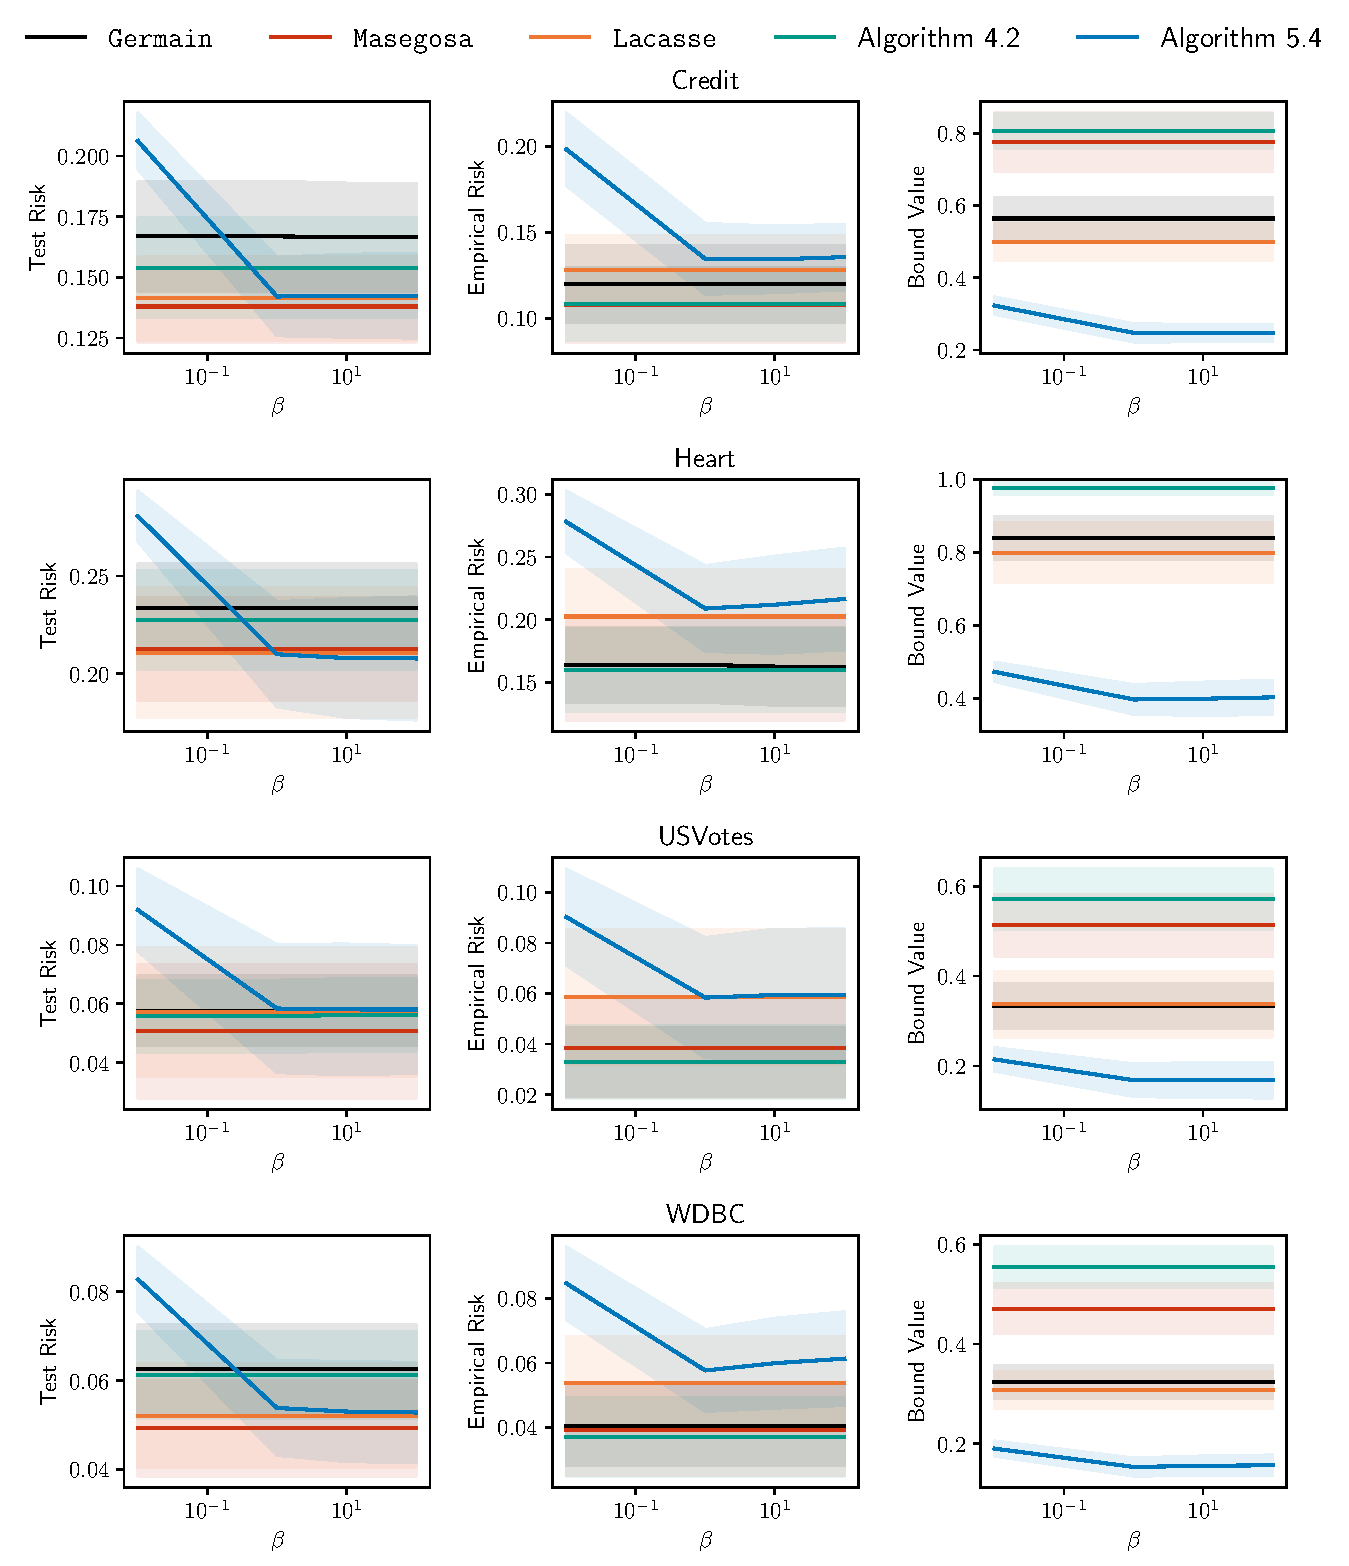
\includegraphics[width=\textwidth]{chapter_5/figures/prior_1.pdf}
    \caption{
    Plot of the impact of the prior $\paramDirP$ on the performance of the stochastic majority vote.
    More precisely, the x-axis represents the value of all the parameters $\sparamDirP_j$ with $j\in\{1,\dots,\card(\H)\}$ and the y-axis are the values of the test risks, the empirical risks or the bound values.
    The mean (plain lines) and the standard deviations (shadows) are obtained for all values on 10 runs.
    }
    \label{ap:mv-sto:fig:prior-1}
\end{figure}

\begin{figure}
    \centering
    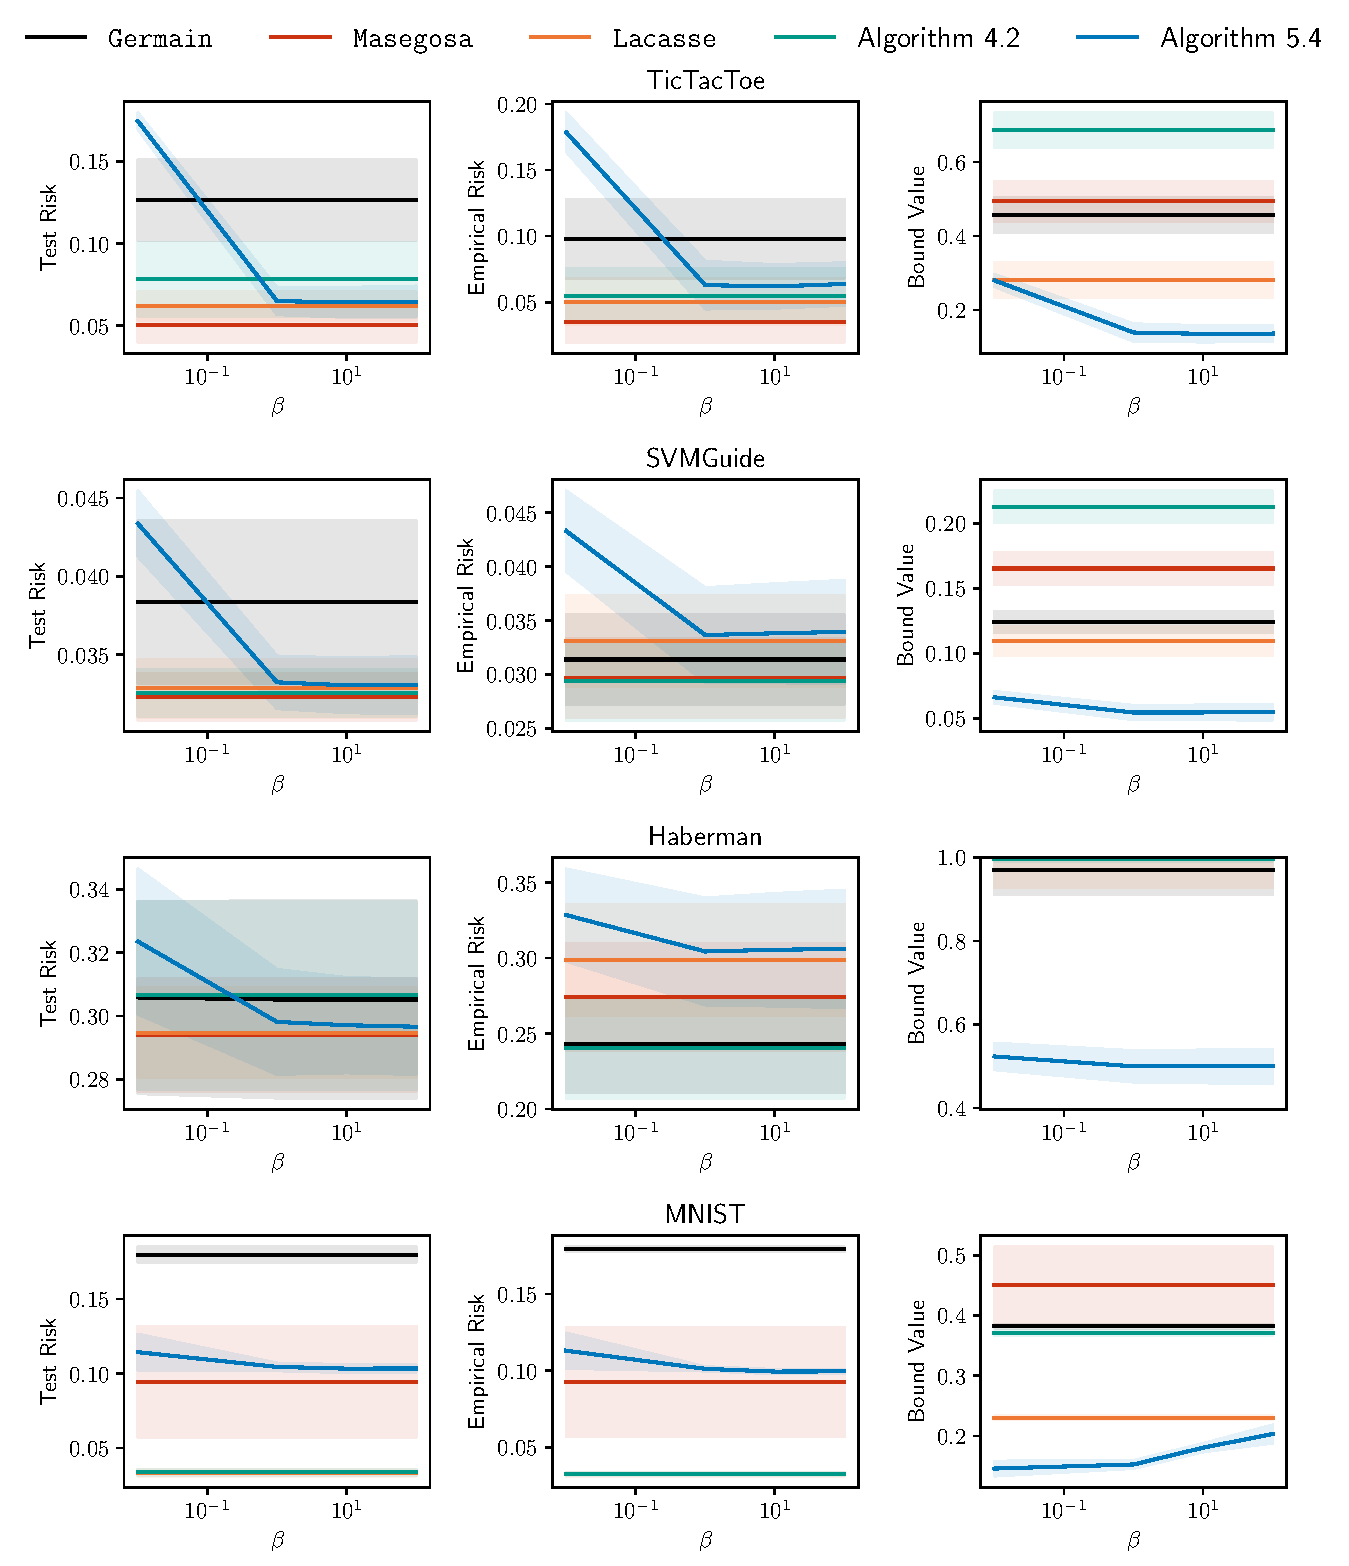
\includegraphics[width=\textwidth]{chapter_5/figures/prior_2.pdf}
    \caption{
    Plot of the impact of the prior $\paramDirP$ on the performance of the stochastic majority vote.
    More precisely, the x-axis represents the value of all the parameters $\sparamDirP_j$ with $j\in\{1,\dots,\card(\H)\}$ and the y-axis are the values of the test risks, the empirical risks or the bound values.
    The mean (plain lines) and the standard deviations (shadows) are obtained for all values on 10 runs.
    }
    \label{ap:mv-sto:fig:prior-2}
\end{figure}

\begin{figure}
    \centering
    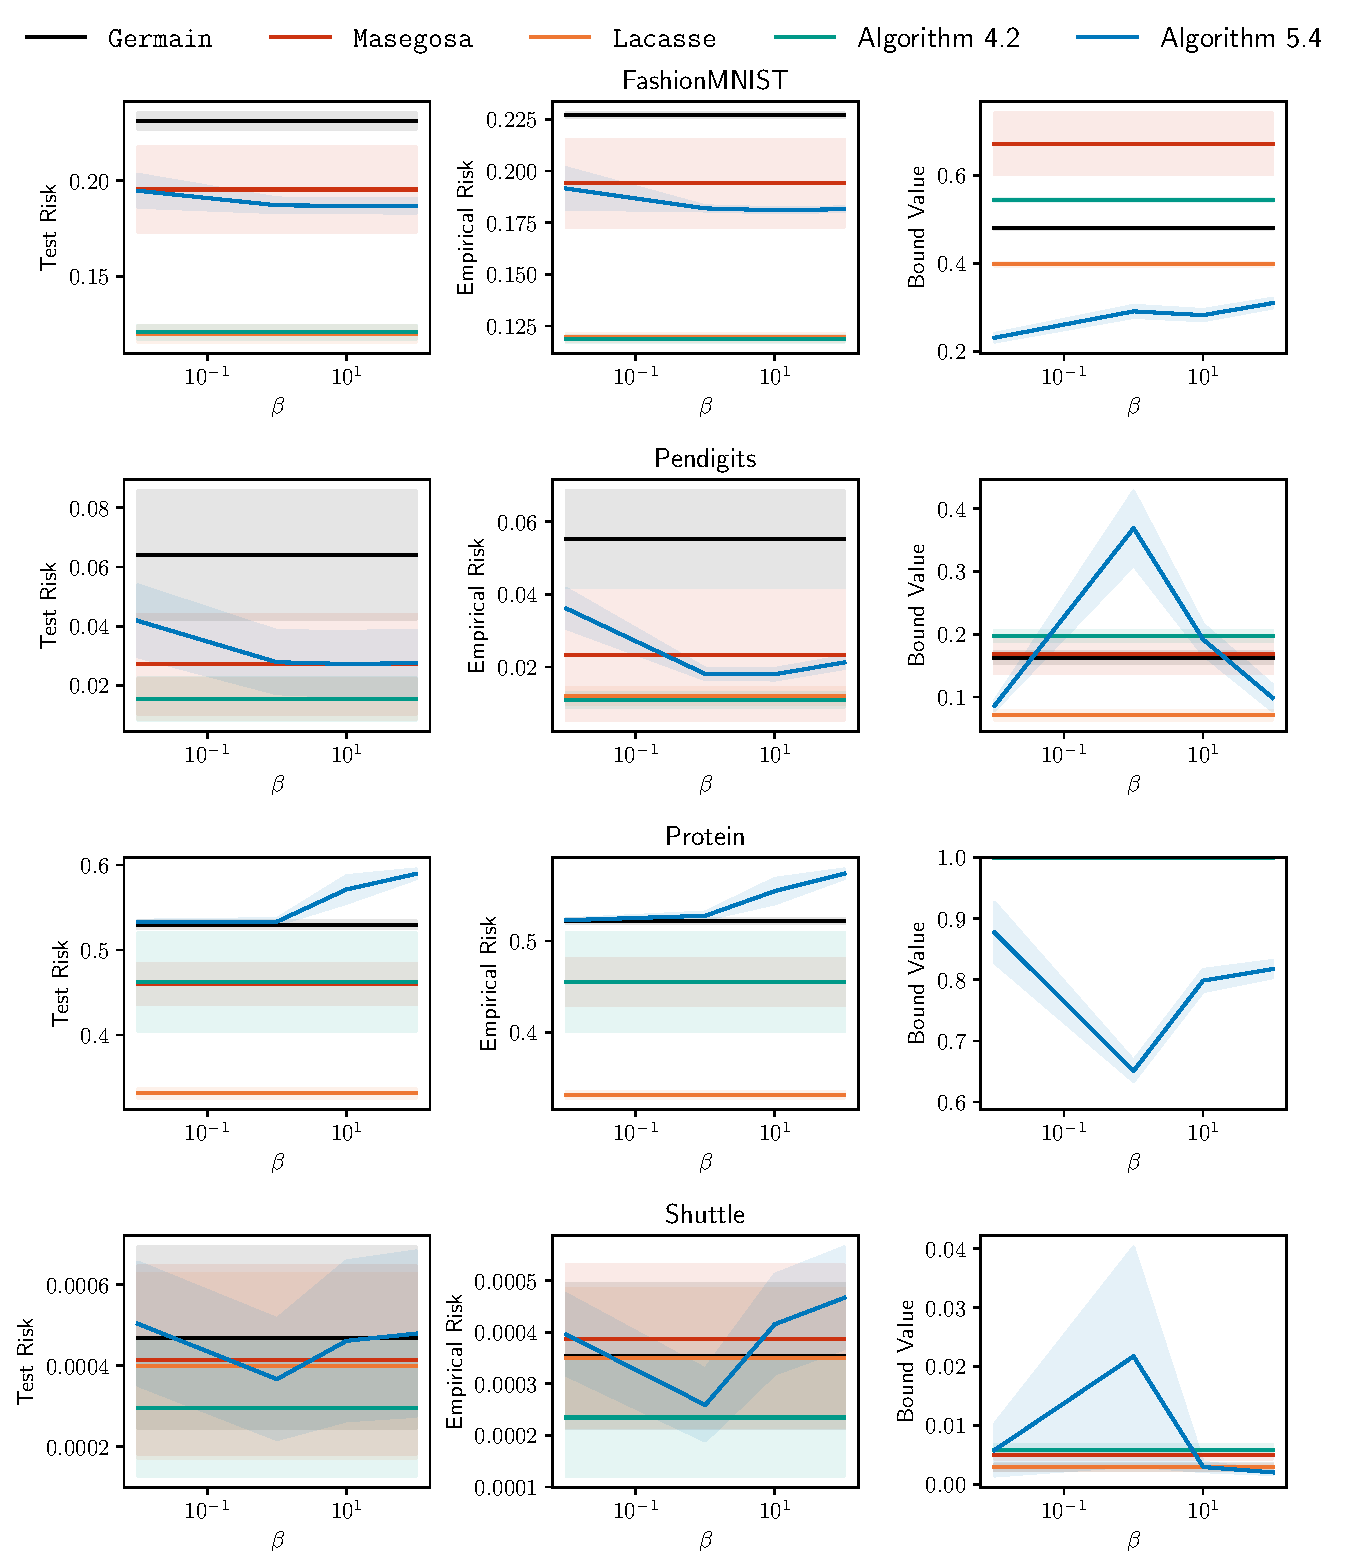
\includegraphics[width=\textwidth]{chapter_5/figures/prior_3.pdf}
    \caption{
    Plot of the impact of the prior $\paramDirP$ on the performance of the stochastic majority vote.
    More precisely, the x-axis represents the value of all the parameters $\sparamDirP_j$ with $j\in\{1,\dots,\card(\H)\}$ and the y-axis are the values of the test risks, the empirical risks or the bound values.
    The mean (plain lines) and the standard deviations (shadows) are obtained for all values on 10 runs.
    }
    \label{ap:mv-sto:fig:prior-3}
\end{figure}

\begin{figure}
    \centering
    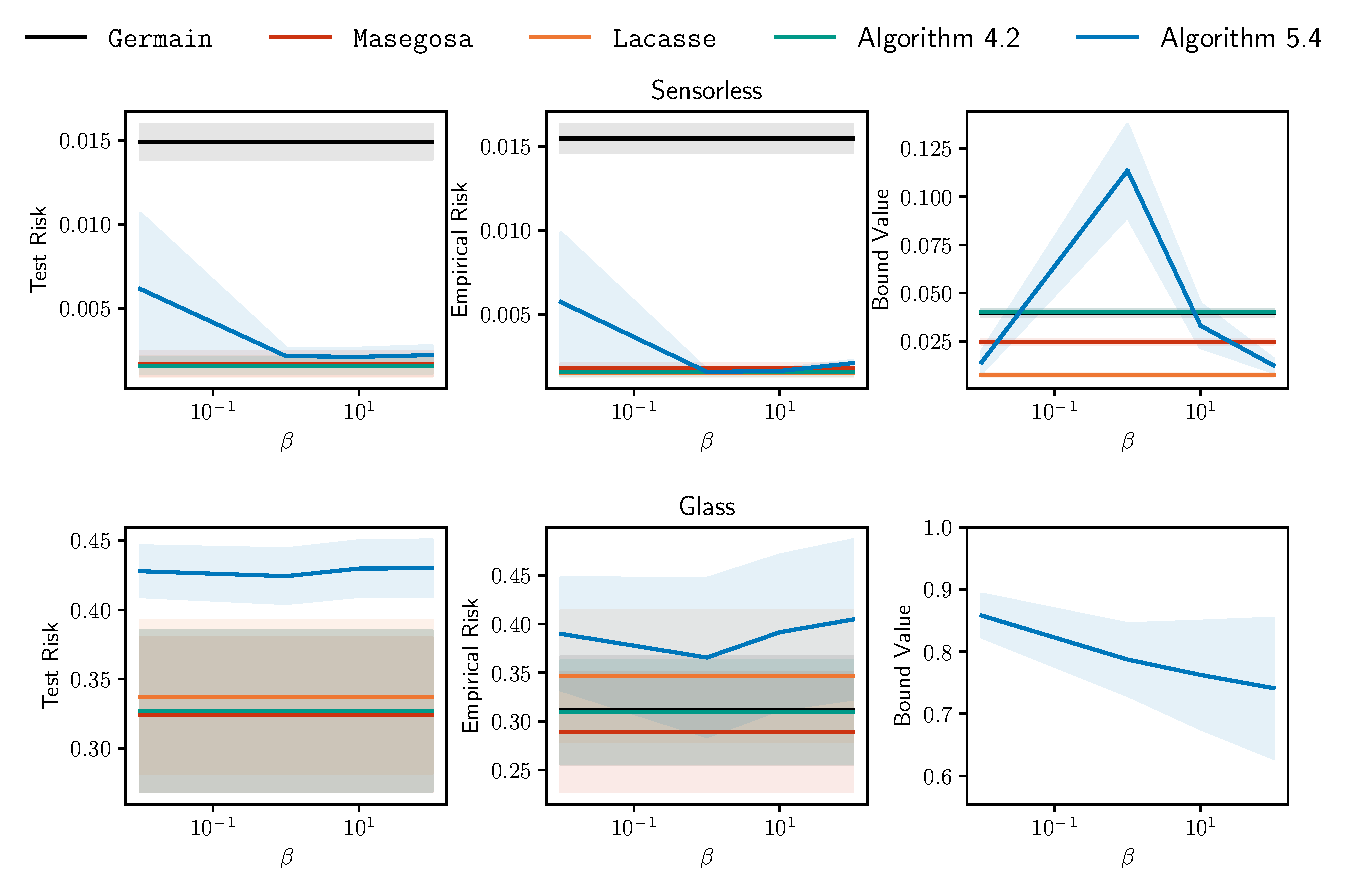
\includegraphics[width=\textwidth]{chapter_5/figures/prior_4.pdf}
    \caption{
    Plot of the impact of the prior $\paramDirP$ on the performance of the stochastic majority vote.
    More precisely, the x-axis represents the value of all the parameters $\sparamDirP_j$ with $j\in\{1,\dots,\card(\H)\}$ and the y-axis are the values of the test risks, the empirical risks or the bound values.
    The mean (plain lines) and the standard deviations (shadows) are obtained for all values on 10 runs.
    }
    \label{ap:mv-sto:fig:prior-4}
\end{figure}

\begin{figure}
    \centering
    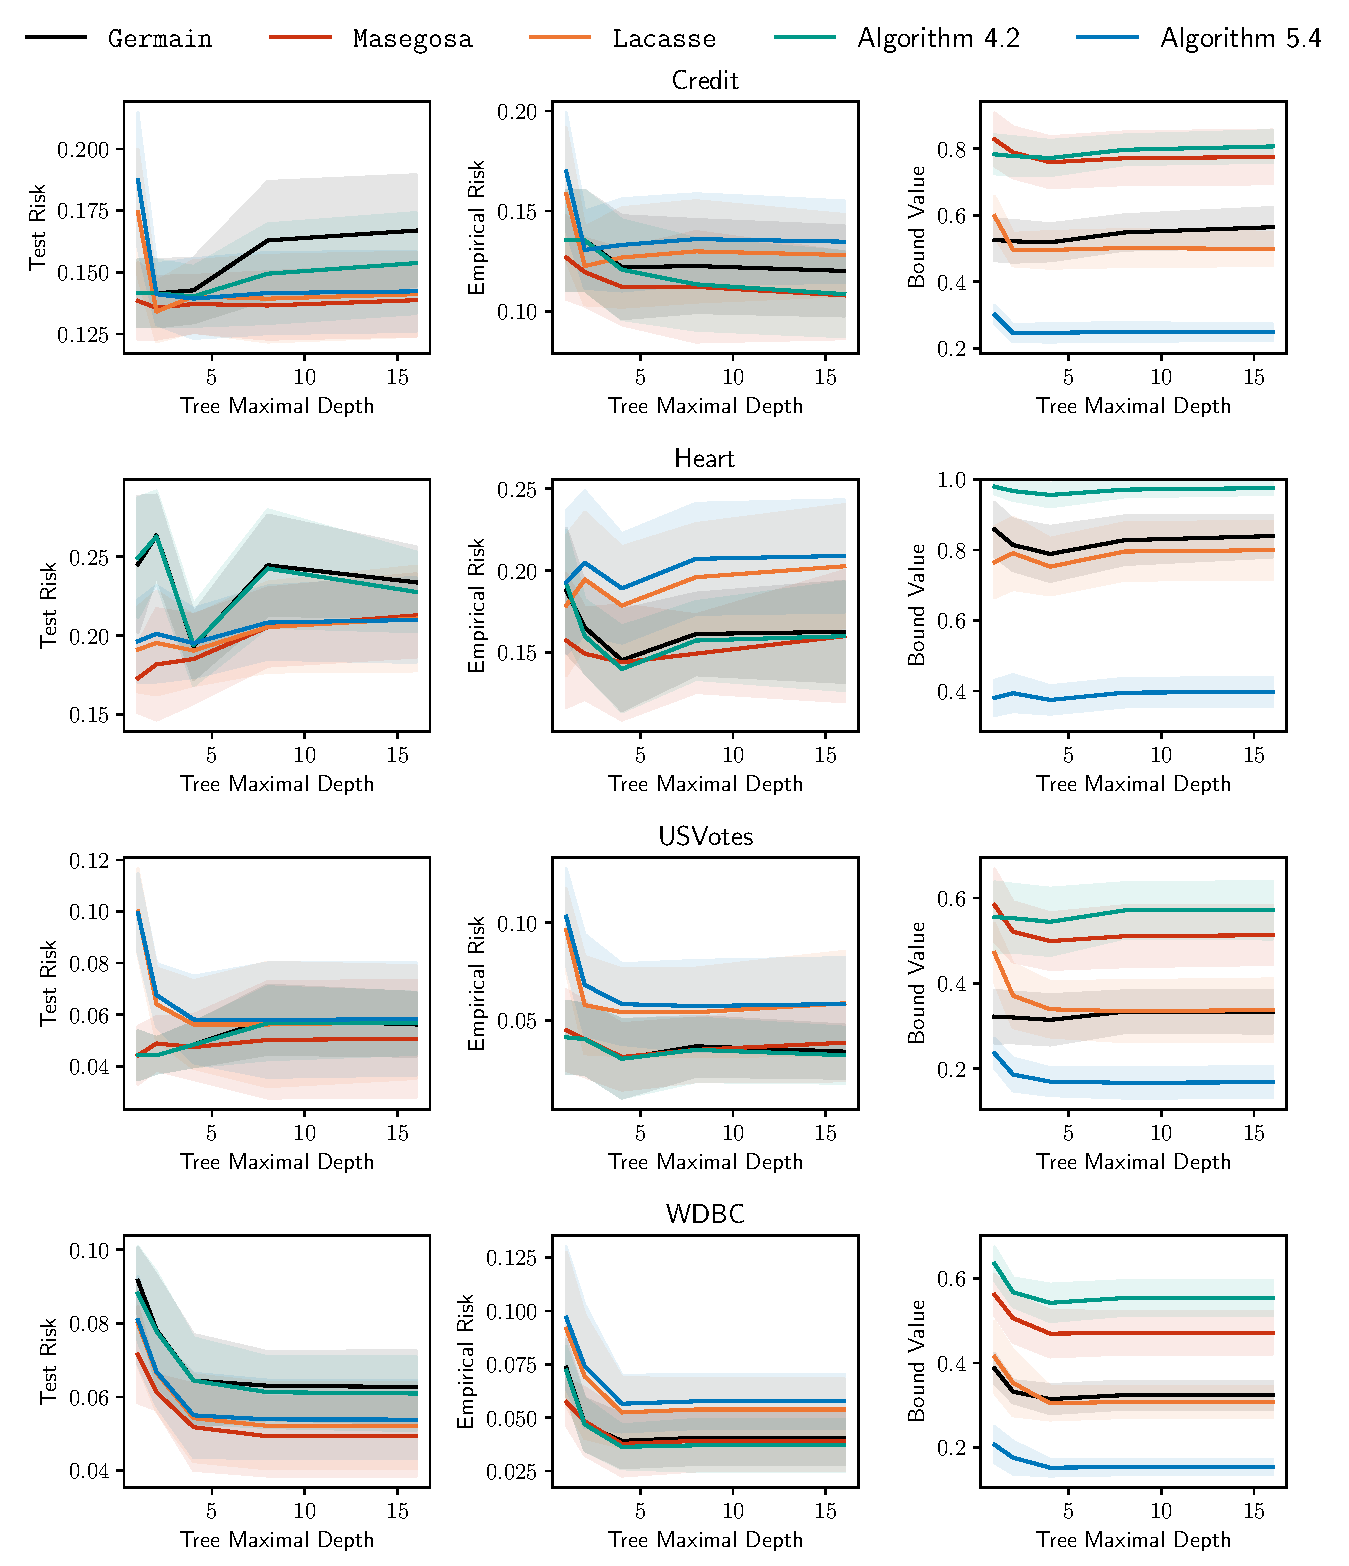
\includegraphics[width=\textwidth]{chapter_5/figures/depth_1.pdf}
    \caption{
    Plot of the impact of tree maximal depth on the performance of the stochastic majority vote.
    More precisely, the x-axis represents the value of the tree maximal depth and the y-axis are the values of the test risks, the empirical risks or the bound values.
    The mean (plain lines) and the standard deviations (shadows) are obtained for all values on 10 runs.
    }
    \label{ap:mv-sto:fig:depth-1}
\end{figure}

\begin{figure}
    \centering
    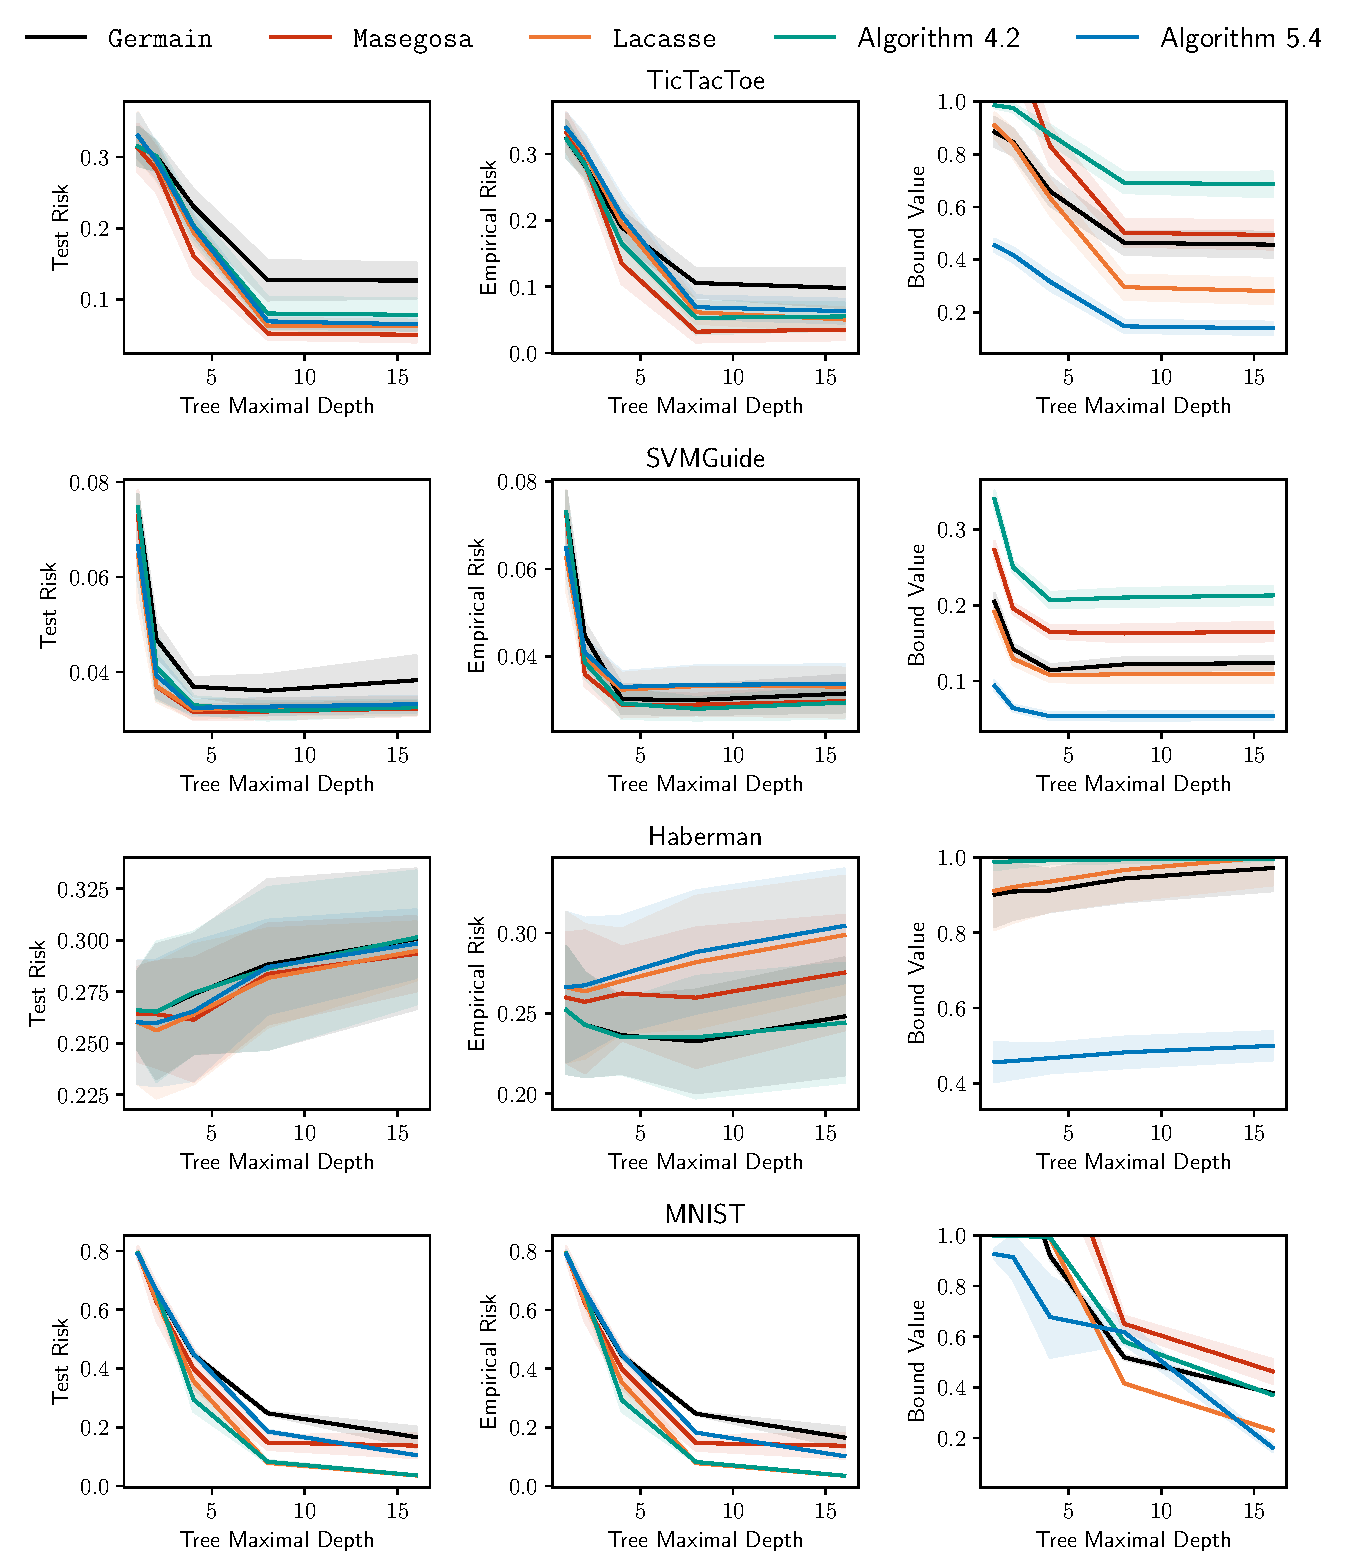
\includegraphics[width=\textwidth]{chapter_5/figures/depth_2.pdf}
    \caption{
    Plot of the impact of tree maximal depth on the performance of the stochastic majority vote.
    More precisely, the x-axis represents the value of the tree maximal depth and the y-axis are the values of the test risks, the empirical risks or the bound values.
    The mean (plain lines) and the standard deviations (shadows) are obtained for all values on 10 runs.
    }
    \label{ap:mv-sto:fig:depth-2}
\end{figure}

\begin{figure}
    \centering
    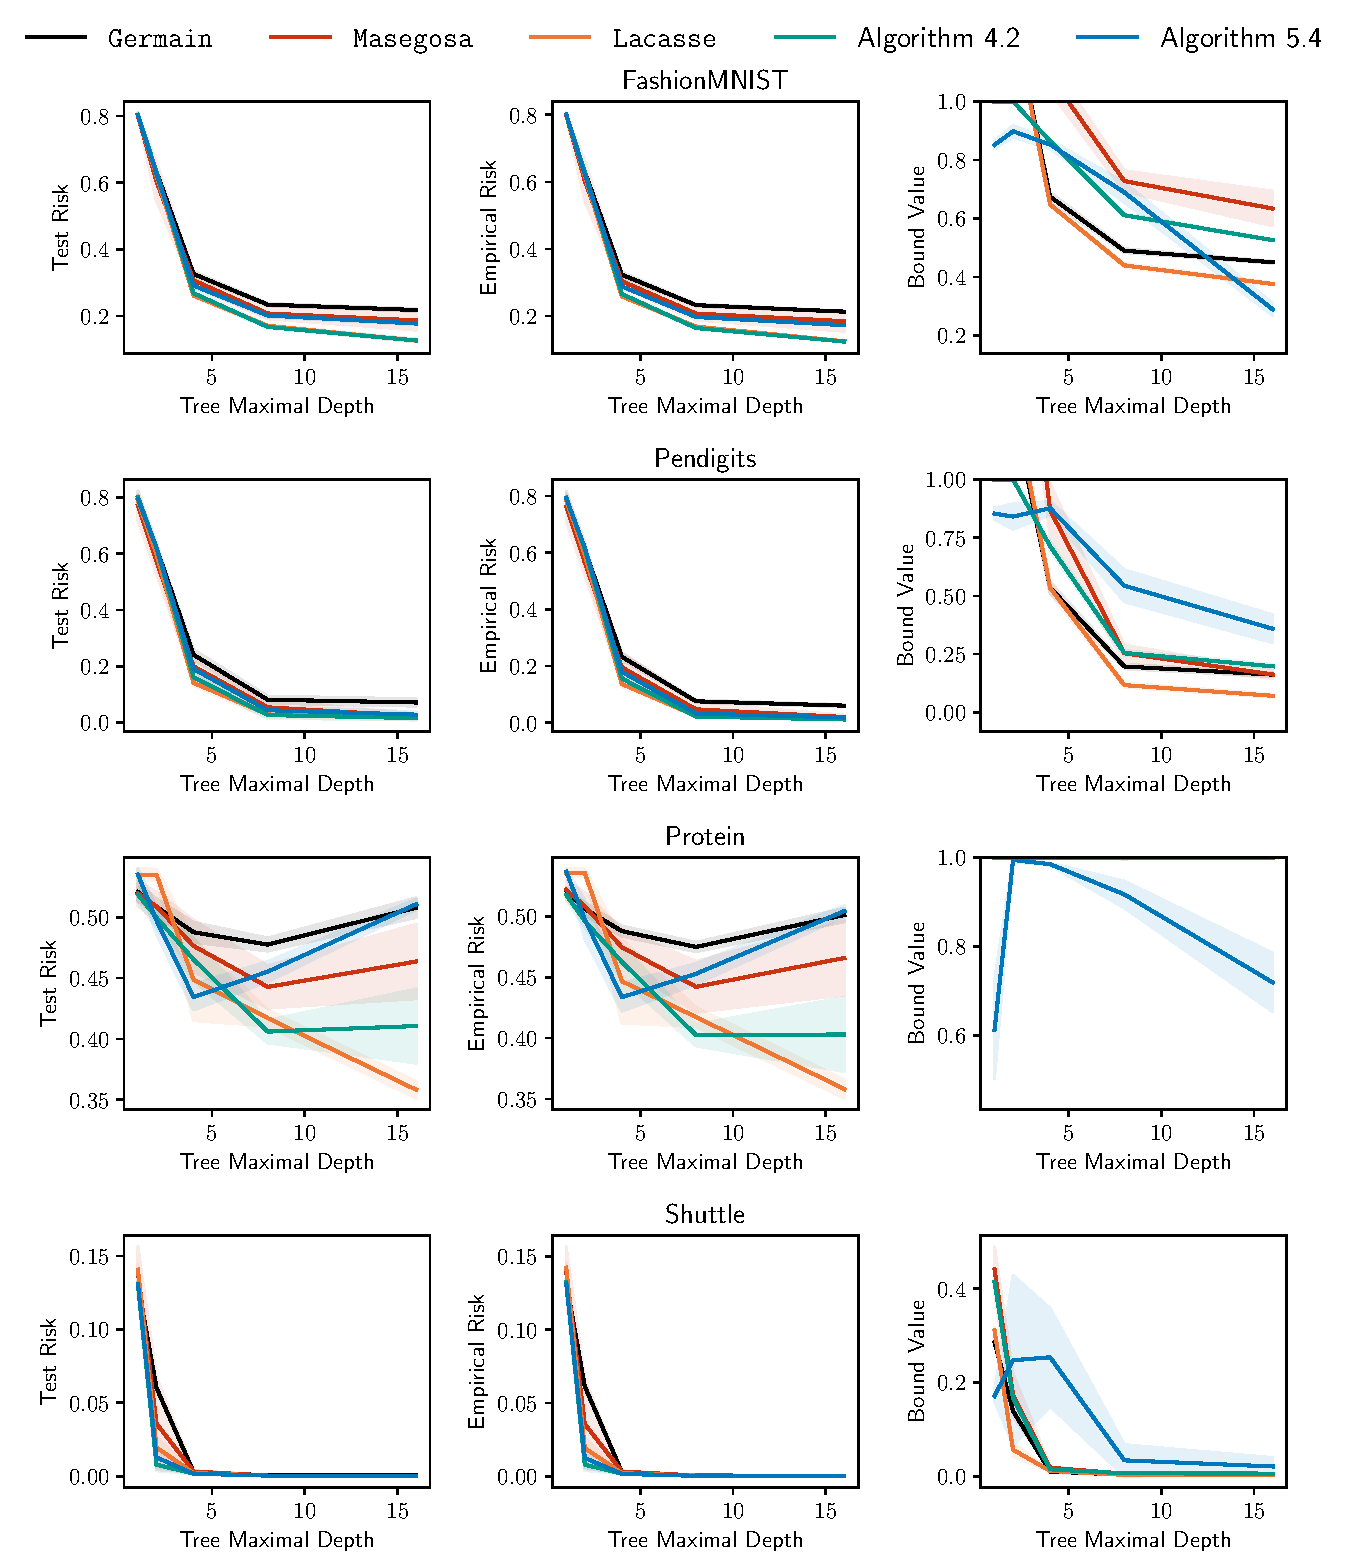
\includegraphics[width=\textwidth]{chapter_5/figures/depth_3.pdf}
    \caption{
    Plot of the impact of tree maximal depth on the performance of the stochastic majority vote.
    More precisely, the x-axis represents the value of the tree maximal depth and the y-axis are the values of the test risks, the empirical risks or the bound values.
    The mean (plain lines) and the standard deviations (shadows) are obtained for all values on 10 runs.
    }
    \label{ap:mv-sto:fig:depth-3}
\end{figure}

\begin{figure}
    \centering
    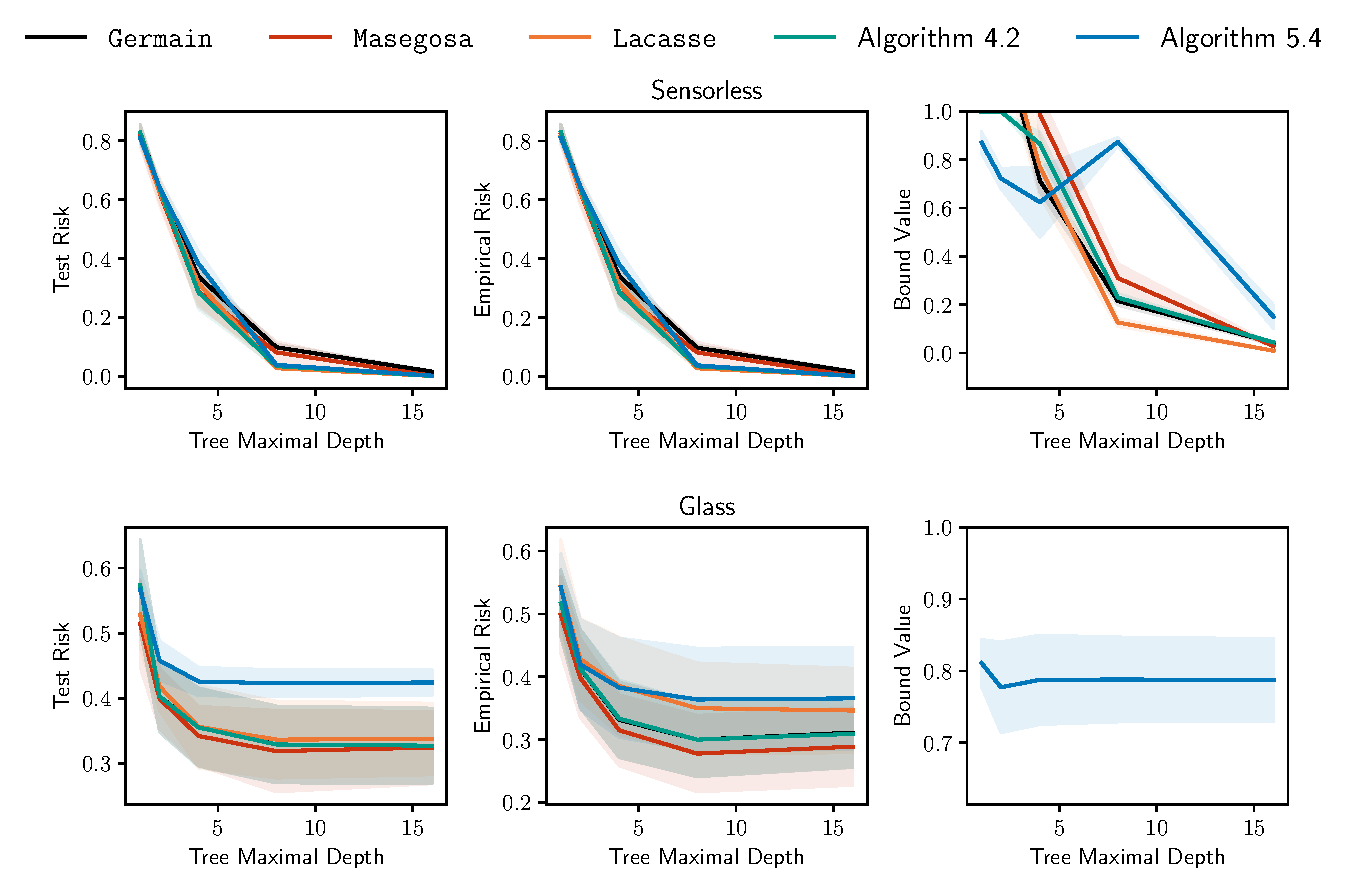
\includegraphics[width=\textwidth]{chapter_5/figures/depth_4.pdf}
    \caption{
    Plot of the impact of tree maximal depth on the performance of the stochastic majority vote.
    More precisely, the x-axis represents the value of the tree maximal depth and the y-axis are the values of the test risks, the empirical risks or the bound values.
    The mean (plain lines) and the standard deviations (shadows) are obtained for all values on 10 runs.
    }
    \label{ap:mv-sto:fig:depth-4}
\end{figure}


\end{noaddcontents}

